\documentclass[sigconf,anonymous,review]{acmart}
\usepackage{booktabs}
\usepackage{amsmath}
\usepackage{array}
\graphicspath{{figures/}{../figures/}{event-completion/figures/}}
\setlength{\emergencystretch}{1em}
\setcopyright{none}
\settopmatter{printacmref=false}
\acmConference[SAC '27]{ACM Symposium on Applied Computing}{April 5--9, 2027}{Gwangju, Republic of Korea}
\acmYear{2027}
\acmDOI{}
\acmISBN{}
\title[Endpoint Inference under Compatible Histories]{Endpoint Inference under Compatible Histories: A Theory-Driven Event Benchmark for Language Models}
\author{Anonymous Author(s)}
\begin{document}
\begin{abstract}
A progressive description alone leaves a bounded endpoint unresolved; sufficient witnessed activity establishes occurrence. We operationalize this distinction using compatible histories and a same-verb benchmark crossing VP composition, contextual evidence and ordinary, defined-nonce and explicit-process presentations. Theory-derived gold is conditional on the stipulated interpretations, without human annotation. Six systems are evaluated on 120 matched families (2,160 core items each), with original-benchmark replication, label controls and paired robustness diagnostics. Three systems solve every explicit-process item; others still reject witnessed activity or confuse unknown with contradiction. Defined nonce predicates can substantially impair performance despite preserving the oracle labels. Negative completion-score contrasts coexist with categorical errors, and none of six structural-guidance accuracy gains survives the prespecified 30-test Holm correction. On an identical 30-family stress subset, DeepSeek solves every explicit-process item but recognizes only 14/30 ordinary-language unknown targets. A supervised unigram diagnostic additionally shows strong surface recoverability. The results support jointly auditing categorical error types, subjective target-truth scores and presentation burden, rather than interpreting one completion-bias statistic as evidence of event-semantic competence.
\end{abstract}
\ccsdesc[500]{Computing methodologies~Natural language processing}
\keywords{event semantics, natural language inference, imperfective paradox, compositionality, theory-derived benchmark}
\maketitle
\section{Introduction}
Whether an event description has a required endpoint cannot generally be read off its verb alone. Drinking water and drinking an entire measured portion share a predicate while differing in the target's extent; walking along a path and walking to its marked end share a motion verb while differing in the required path goal. Inferring a completed bounded event from an ongoing description therefore tests the interaction of predicate, argument structure and contextual evidence. An activity target instead asks whether sufficient activity occurred. Describing both targets as event completion obscures this difference.

The imperfective paradox motivates a useful diagnostic: an ongoing bounded process need not have culminated. Recent language-model work evaluates progressive-to-simple-past inference on ImperfectiveNLI~\cite{ma2026}. A subsequent critique identifies disputed interpretations, interruption ambiguities and prior same-verb comparisons~\cite{han2026}. Same-verb pairing alone is consequently not our novelty. We combine such pairing with compatible-history gold, an explicit occurrence--culmination distinction, three presentations of matched process structure and evidence that separates unspecified outcomes from negative facts.

Gold is conditional on a specified event interpretation, without independent human validation or prior ratings. Presentation differences also involve definitions, notation and length, so they cannot isolate parametric knowledge. The intended-prior module tests a defeasible completion-burden hypothesis rather than a validated causal manipulation.

We contribute (1) a finite compatible-history specification separating occurrence, culmination and unresolved outcomes; (2) a seeded, same-verb matched benchmark crossing composition, presentation and outcome evidence; and (3) a reproducible contemporary evaluation with label controls, probability scores and paired robustness diagnostics. These contributions concern a controlled diagnostic rather than a new general theory of aspect.

The frozen evaluation addresses eight questions: contemporary original-benchmark replication; sensitivity to same-verb VP composition; intended-prior sensitivity; ordinary/nonce differences; explicit-process recovery; contextual override; within-Qwen size associations; and semantic-rule interventions. These are empirical questions about named systems. Event theory supplies normative labels, not a theorem about which architecture or size will perform better.

\section{Background and Related Work}
\subsection{Composition and Event Structure}
Vendler's aspectual distinctions~\cite{vendler1957} and later work on temporal interpretation~\cite{moens1988} provide a foundation for distinguishing activities from endpoint-dependent descriptions. Krifka's account of nominal reference and temporal constitution~\cite{krifka1998} motivates treating theme quantity and progress through that theme compositionally. Our manipulation strata concern quantity, goal paths and incremental coverage. They indicate where an endpoint requirement changes; they are not independent theoretical mechanisms. Here boundedness means a required culmination, not merely a finite observation interval. The reporting horizon does not give the activity target an inherent terminal state.

We use a finite interpretation of each single episode rather than treating the past tense as an unrestricted existential over the agent's lifetime. Cancellation explicitly rules out attainment and resumption by the reporting horizon. Destruction after attainment leaves past completion true. Sufficient nonzero activity is asserted so that preparation or onset is not mistaken for completed activity occurrence.

\subsection{Imperfective Inference and Benchmark Validity}
Ma and Miyao introduce ImperfectiveNLI with 400 items in four groups~\cite{ma2026}. Its published labels remain unchanged in our replication. Han and Sun's critique~\cite{han2026} motivates treating original-gold accuracy and disputed interpretations separately. Their supplied exclusion list retains 303 items; an additional Group A flag identifies 76 items without explicit noncompletion. Those are published concern flags rather than new independent annotations. We report the full original pool, the published filtered pool and the explicit-noncompletion subset, with denominators.

\subsection{Context and Controlled Semantic Diagnostics}
Pru\'{s} et al.~\cite{prus2024,prus2025} show that nonexpert aspectual judgments are not exhausted by aspect classes and that added context resolves some, but not all, disagreement. Their results motivate separating stipulated entailments from plausible outcomes. Our probability module does not substitute model scores for human beliefs.

CoRE~\cite{core2025} evaluates ongoing/completed descriptions with and without story context, including an unsure option; contextual benefits vary across its evaluated systems. CxMP~\cite{cxmp2026} tests constructional meanings through controlled minimal pairs and includes pseudoword substitution. Thus neither context-conditioned event reasoning nor lexical replacement is novel here. Our defined nonce predicates preserve an explicit process relation, unlike replacing content words with uninterpreted pseudowords. We examine matched endpoint truth alternatives across all presentations.

COGS~\cite{cogs2020} evaluates lexical and structural generalization, while HANS~\cite{hans2019} illustrates that NLI accuracy can reflect superficial heuristics. We therefore report a held-out renderer and exploratory word-unigram baselines trained on disjoint pilot gold. These supervised baselines have different information from zero-shot language models and serve as surface-recoverability diagnostics, not a fair model leaderboard.

\section{Methodology}
\subsection{Compatible-History Predictions}
Let $\mathcal{H}(P)$ be the nonempty set of histories compatible with premise $P$. For target $T$, define entailment ($E$), contradiction ($C$) and unknown ($U$) by
\begin{equation}
 L(P,T)=\begin{cases}
 E & \forall h\in\mathcal{H}(P):T(h),\\
 C & \forall h\in\mathcal{H}(P):\neg T(h),\\
 U & \text{otherwise}.
 \end{cases}
\end{equation}
A bounded target $B(h)$ requires attainment of progress state 4. An occurrence target $A(h)$ requires the stated sufficient activity witness, represented by at least two progress stages. Neutral evidence permits both $(1,2,S)$ and $(1,2,3,4,S)$, where $S$ denotes permanent stopping. Supporting evidence permits only the latter; cancellation permits only the former. The two histories are representatives of the endpoint truth alternatives, not an empirical event-frequency distribution.

\begin{table}[t]
\centering
\caption{Normative predictions, identical across the three matched presentations. These are theory-derived labels, not observed model accuracies.}
\label{tab:theory}
\setlength{\tabcolsep}{3pt}
\begin{tabular}{lccc}
\toprule
Evidence & \shortstack{Bounded\\target} & \shortstack{Activity\\target} & $q(B)-q(A)$\\
\midrule
Neutral & $U$ & $E$ & $[-1,0]$\\
Endpoint attained & $E$ & $E$ & $0$\\
Permanent cancellation & $C$ & $E$ & $-1$\\
\bottomrule
\end{tabular}
\end{table}

The probability columns presuppose a coherent target-truth assessment accepting the premise. A neutral bounded target has no theory-specified point probability. A strict negative neutral contrast requires a nondegenerate endpoint belief; logic gives only the weak inequality. A highly probable unknown target remains unknown as a categorical entailment judgment. No threshold maps the elicited score into a label.

\subsection{Families, Gold and Splits}
A seeded generator allocates 120 main families and 40 disjoint pilot families, with 12 real lemmas and three manipulation strata. Each main lemma has ten scenario realizations. Family counts therefore exceed independent lexical and process-mechanism counts. Repeated names, objects and underlying progress rules do not constitute independent semantic mechanisms.

Each family crosses three presentations, bounded/activity targets and neutral/supportive/cancelling evidence, producing 18 items. Gold comprises 12 entailed, three contradicted and three unknown items per family. We preserve this semantic imbalance and report macro-label and cell accuracy rather than forcing equal labels by changing targets. Original and generated pairs undergo exact/normalized overlap checks. Automatic checks verify allocation, shared lemmas and nonce forms, process predicates and the truth matrix. Gold never comes from model responses.

The agent, underlying theme or path, and episode horizon are matched within a pair. A bounded theme is the entire stipulated portion or text, or a marked path goal. The activity counterpart requires sufficient witnessed processing. Quantity items exclude additional target quantities; cancellation excludes endpoint attainment and later continuation within the same episode. Every generated item is marked as not human validated. The theory-derived predictions agree with all 5,744 item variants and controls in the main freeze. This includes planned robustness renderings, not 5,744 independent families.

\begin{table}[t]
\centering
\caption{VP excerpts from frozen Real targets (F001, F057 and F141). The full hypotheses retain the same agent, episode and reporting horizon.}
\label{tab:vp_examples}
\setlength{\tabcolsep}{3pt}
\begin{tabular}{@{}l>{\raggedright\arraybackslash}p{.40\columnwidth}>{\raggedright\arraybackslash}p{.34\columnwidth}@{}}
\toprule
Verb & Bounded argument & Activity argument\\
\midrule
drink & exactly one measured glass of water & water\\
walk & to the marked far end of the corridor & along the corridor\\
read & the entire specified paragraph & text from the specified paragraph\\
\bottomrule
\end{tabular}
\end{table}

Matching preserves the underlying episode and endpoint truth alternatives, rather than making complete premises differ by a single word. Bounded Real items additionally exclude surplus targets; their outcome evidence names the required quantity, goal or coverage. Activity evidence states witnessed occurrence and duration. These task-specific wording differences restrict attribution of a contrast to composition alone. Explicit endpoint and cancellation sentences can directly establish target truth; performance here does not demonstrate recovery of implicit event outcomes from unrestricted discourse.

\subsection{Presentations and Intended Priors}
Real uses ordinary verbs and arguments. Nonce supplies a shared neutral process definition and changes its arguments within the same predicate root. Micro supplies an explicit symbolic process and target rule. The process relation and evidence are matched within family. Length, definition burden, notation and lexical associations remain different. A Real-definition control helps diagnose information-load effects but does not identify a causal internal knowledge component. Dictionary noncollision of nonce forms cannot establish absence from all training data.

A separate Real-bounded module uses 40 main families with two intended completion-burden levels and three contexts, yielding 240 items per model. Smaller portions, shorter texts and nearer goals motivate a hypothesis of higher neutral completion plausibility, conditional on otherwise comparable processing. No independent prior ratings were collected. Direction and effect size are therefore not validated. Explicit endpoint and cancellation evidence dominate the logical label regardless of the burden cue. Intended-prior effects remain exploratory.

\subsection{Models and Collection}
Six named systems are fixed before main core outcomes: Qwen3 at 8B, 14B and 32B; Llama 3.1 8B Instruct; Ministral 8B 2512; and Gemma 3 12B IT. A 30-family core and 20-family intended-prior subset is reserved for DeepSeek-V3.2 stress evaluation. Its different population and MoE architecture prevent pooling it into dense-size regression.

OpenRouter providers are fixed: Alibaba for Qwen8, Groq for Llama8, Mistral for Ministral8, and DeepInfra BF16/FP8/FP4 endpoints for Gemma, larger Qwen and DeepSeek respectively. Qwen dense parameter counts are 8.2, 14.8 and 32.8 billion. Size associations are limited by supplier, precision and training differences; three sizes do not establish a scaling law or transition.

Requests use temperature zero, top-$p$ one, a 256-token output budget, no tools and no requested reasoning trace. Explicit gateway disable controls and the Qwen-supported \texttt{/no\_think} switch address supplier-specific hidden reasoning. Usage metadata, including residual wrapper tokens, remains recorded. The Qwen switch is applied uniformly across its three sizes and is a disclosed adaptation of the original zero-shot prompt. Non-Qwen original prompt bodies are unchanged. This is a contemporary protocol adaptation rather than exact reproduction of historical models.

Generated tasks request a short JSON judgment and subjective hypothesis probability. Label-only controls omit the latter. Successful outputs, including parse errors, are never retried. Only failed transport requests may be resumed. Full request hashes include messages, model, supplier and decoding; exact equivalents reuse the same response and are not independent stochastic replicates. All planned analysis cells remain represented, including missing outcomes.

\subsection{Pilot, Freeze and Robustness}
The disjoint two-system pilot has 1,600 valid responses (720 core, 60 prior and 20 label controls each). A 40-call schema check motivated removal of a redundant probability field; both versions are retained. Pilot event families and prior items are excluded from main event estimates and never used for effect-based item/model selection. Twenty generic Llama label-control payloads recur identically in the main diagnostic control set and reuse their pilot responses; they are not fresh independent trials. Matching endpoint-control payloads are likewise cached. The local freeze precedes main core collection and is not external preregistration.

A seeded 24-family robustness subset crosses the three presentations, two targets and neutral/cancelling evidence. The six paired variants are label order, held-out renderer, name replacement, label-only output, natural guidance and structural guidance. The Real-definition control changes only Real, requiring 96 additional cells per model; unchanged artificial baselines are reused. A new renderer is a limited paraphrase diagnostic rather than open-domain generalization. Original replication and all robustness cells retain their planned denominators. A post-freeze supplementary wording control repairs the 30 known passive-participle defects on all six main systems (180 cells), holding hypotheses and gold fixed. It retains original responses and adds no confirmatory tests; later collection and service variation restrict causal attribution.

\subsection{Metrics and Statistics}
We report all-planned accuracy, parse-valid accuracy, macro-label accuracy, and bounded entailment error rates by evidence. Subjective $q$ measures target truth, not entailment probability or calibrated risk. Compositional sensitivity is $q(B)-q(A)$, with matched categorical contrasts alongside it. Intended-prior sensitivity is a paired high-minus-low score, not proof of an internal knowledge mechanism. A score gap accompanied by correct labels is not itself a logical error. Conversely, a negative neutral score contrast can coexist with incorrectly calling the bounded target contradicted. The score contrast cannot certify categorical correctness.

Five prespecified contrasts per main model form one 30-test Holm family: Real neutral compositional sensitivity; its Real--Nonce and Real--Micro differences; Real bounded cancellation-minus-neutral $q$; and structural-rule accuracy gain. Family contrasts use 10,000 seeded bootstrap draws that resample verbs and then families within verbs. Block sign-flip tests assume exchangeable effect signs across lexical blocks under the contrast null; only 12 blocks limit resolution and generalization. These intervals concern resampling the lexical/family set, not service stochasticity or arbitrary English constructions. Family-only bootstrap is a sensitivity analysis. Reported 95\% intervals are marginal; multiplicity correction applies to the p-values. Rule gains retain parse/transport failures as incorrect; probability contrasts use complete pairs with adverse missing-score bounds.

Binary mixed-effects analysis follows the prespecified interaction of composition, presentation and context, with effects for stratum and template, a family intercept and slope, and a verb intercept. Linear mixed models on raw $q$ are secondary. Singular or separated fits are disclosed, simplified only as specified, and replaced by cell/clustered contrasts when not estimable. Ordinary beta regression is inappropriate at exact zero/one scores; no silent clipping is performed. Within-Qwen size analyses remain descriptive associations. 

\subsection{Reproducibility}
The anonymous review archive retains generated stimuli, theory predictions, complete response/attempt ledgers, all 30 primary and 380 secondary diagnostics, model-fit failures, source-data hashes, editable figures and offline analysis scripts. Frozen stimulus replay is byte-identical in a disposable checkout. API credentials, unlicensed upstream code and third-party full texts are excluded; source acquisition instructions and unchanged original-dataset attribution are retained. The local freeze is auditable but is not external preregistration.

\subsection{Implementation and AI Assistance}
Codex assisted design refinement, template and generator implementation, literature auditing, experimental orchestration, analysis code, figures and manuscript drafting. Labels are computed by the published finite-history rules rather than sampled from a generative model. Empirical observations come from recorded API calls. No human annotations or prior ratings exist.

\section{Results}
\subsection{Collection and Label Controls}
The completed main collection represents 28,104 planned cells across the six systems, corresponding to 27,984 unique requests. All have valid parsed outcomes. Of the unique requests, 35 reuse matching pilot or endpoint-control responses; 120 additional planned cells reuse equivalent requests. Transport failures remain in the attempt ledger, and resumed requests do not constitute independent trials. The fixed 660-cell strong-model stress collection is also complete. All 180 supplementary grammar responses are also complete. The completed-main contrast estimates use the unchanged frozen 30-test specification. Known returned charges total \$0.9224; conservative reserves for unavailable billing bring the project ledger to \$2.0425, below the \$10 target.

All systems answer the generic entailed and contradicted controls correctly (20/20 each). Five also answer every generic unknown control correctly. Qwen8 answers none of its 20 generic unknown controls correctly, yet answers all 120 Micro unknown items correctly. Its failures therefore depend on presentation and task wording; they do not establish an absolute inability to use the unknown label. Conversely, successful generic controls do not prevent event-specific unknown errors.

\begin{table*}[t]
\centering
\caption{Completed main core results (percent). Each presentation has 720 items per system: 480 entailed, 120 contradicted and 120 unknown. Acc. uses all planned cells; macro averages the three label recalls; U is unknown recall. The final column is a separate generic unknown-label control, including the disclosed cached controls. Perfect Micro scores concern supplied finite rules rather than unrestricted language competence.}
\label{tab:core_results}
\setlength{\tabcolsep}{4pt}
\begin{tabular}{lrrrrrrrrrr}
\toprule
 & \multicolumn{3}{c}{Real} & \multicolumn{3}{c}{Nonce} & \multicolumn{3}{c}{Micro} & Generic U\\
System & Acc. & Macro & U & Acc. & Macro & U & Acc. & Macro & U & Correct\\
\midrule
Qwen8 & 91.9 & 83.9 & 65.0 & 59.2 & 54.6 & 0.0 & 100.0 & 100.0 & 100.0 & 0/20 \\
Llama8 & 82.4 & 64.7 & 15.8 & 85.3 & 70.6 & 15.0 & 89.4 & 78.9 & 36.7 & 20/20 \\
Ministral8 & 58.3 & 67.7 & 79.2 & 73.5 & 86.7 & 100.0 & 66.7 & 83.3 & 100.0 & 20/20 \\
Gemma12 & 92.2 & 84.4 & 54.2 & 92.1 & 84.2 & 52.5 & 100.0 & 100.0 & 100.0 & 20/20 \\
Qwen14 & 94.9 & 89.7 & 70.0 & 63.5 & 57.2 & 1.7 & 86.2 & 93.1 & 100.0 & 20/20 \\
Qwen32 & 94.7 & 89.4 & 68.3 & 86.5 & 92.6 & 97.5 & 100.0 & 100.0 & 100.0 & 20/20 \\
\bottomrule
\end{tabular}
\end{table*}

\subsection{Composition, Presentation and Categorical Errors}
\begin{figure*}[t]
\centering
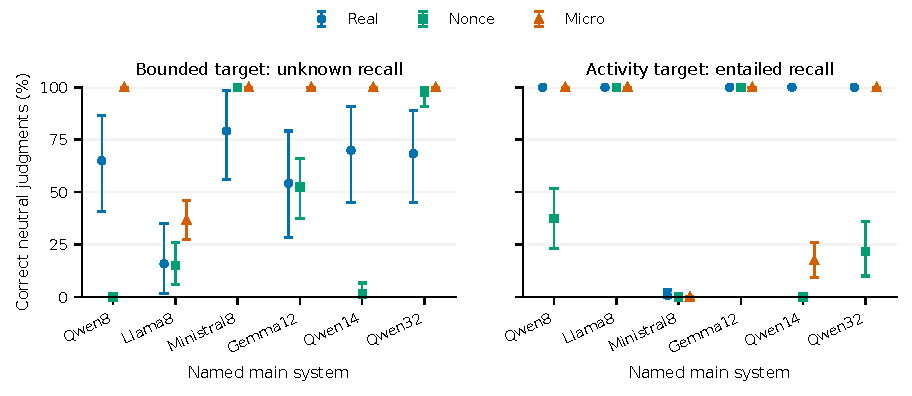
\includegraphics[width=\textwidth]{main_category_accuracy.pdf}
\caption{Neutral categorical diagnostics: unresolved endpoint versus witnessed occurrence. Each point retains 120 planned families; missing/invalid labels count incorrect. Marginal 95\% intervals use 10,000 verb-then-family bootstrap draws over 12 lexical blocks. Floor/ceiling intervals concern the retained construction pool, not service certainty. All six systems and three presentations are shown; no new p-values.}
\label{fig:category}
\end{figure*}
Table~\ref{tab:core_results} shows that aggregate accuracy can conceal label-specific failure. Figure~\ref{fig:category} separates neutral endpoint uncertainty from witnessed activity occurrence. Real accuracy exceeds 91\% for four systems, while their unknown recall ranges from 54.2\% to 70.0\%. Llama8 reaches 82.4\% Real accuracy but only 15.8\% unknown recall. The majority-label proportion is 66.7\%, making macro-label and cell diagnostics necessary.

Nonce substitution does not uniformly improve reasoning. Qwen8 falls from 91.9\% Real accuracy to 59.2\% Nonce accuracy, and Qwen14 from 94.9\% to 63.5\%. Their neutral Nonce activity accuracy is respectively 37.5\% and 0\%, despite that target's explicit occurrence witness. Qwen32 also answers only 21.7\% of neutral Nonce activity targets correctly. Such errors concern whether sufficient activity occurred, rather than only whether a bounded process culminated. Qwen8 calls every neutral Nonce bounded target contradicted; Qwen14 does so on 118/120 items. Their main unknown errors in this presentation therefore cannot be described as excessive completion entailment. These systems perform poorly on the defined-predicate task despite unchanged oracle labels.

Micro yields perfect core accuracy for Qwen8, Gemma12 and Qwen32. It does not provide universal recovery: Llama8 reaches 89.4\%, Qwen14 86.3\%, and Ministral8 66.7\%. Ministral8 correctly identifies every Micro unknown and contradicted item but only half of the entailed items, giving 83.3\% macro accuracy. It fails every neutral Micro activity target. Qwen14 answers 17.5\% of that same cell correctly. The explicit process presentation can therefore localize failures rather than merely produce a higher total score.

All six Real neutral compositional-sensitivity point estimates are negative, ranging from $-0.504$ to $-0.248$. A negative score difference is insufficient evidence of correct categorical inference. Ministral8 has zero mean neutral Nonce and Micro contrast while failing their occurrence targets; Qwen14 has negative neutral Nonce sensitivity despite failing every neutral activity judgment. The score and categorical outcomes must be interpreted jointly.

Explicit cancellation establishes the negative operational label: Real bounded cancellation accuracy is 100\% for Qwen32, 99.2\% for Gemma12 and Qwen14, 86.7\% for Qwen8, 78.3\% for Llama8, and 75.0\% for Ministral8. All systems reach 100\% in the corresponding Micro cell. These statements concern explicitly supplied negative evidence. The retained Real estimates include the known participle defects; the paired repair diagnostic below retains them as baseline observations.

\subsection{Prespecified Clustered Contrasts}
\begin{table*}[t]
\centering
\caption{All 30 prespecified contrasts. Each cell gives estimate, marginal lexical/family bootstrap 95\% CI, and Holm-adjusted $p$ across the complete 30-test family. The first four columns are q differences over 120 complete paired families; the rule column is percentage-point accuracy change over 24 complete families with 12 matched cells each. Exact block sign flips use the retained lexical blocks. Marginal intervals and adjusted tests have different multiplicity scopes. All planned probability contrasts have complete scores, so adverse bounds equal the point estimate.}
\label{tab:primary_results}
\setlength{\tabcolsep}{5pt}
\begin{tabular}{lrrrrr}
\toprule
System & Real CS & Real--Nonce CS & Real--Micro CS & Cancel--neutral q & Structural rule\\
\midrule
Qwen8 & \shortstack{$-0.344$\\$[-0.457,-0.220]$\\$0.043$} & \shortstack{$0.372$\\$[0.235,0.521]$\\$0.015$} & \shortstack{$0.156$\\$[0.043,0.280]$\\$0.279$} & \shortstack{$-0.485$\\$[-0.585,-0.381]$\\$0.015$} & \shortstack{$-0.69$\\$[-2.63,1.09]$\\$1.000$} \\[3pt]
Llama8 & \shortstack{$-0.504$\\$[-0.713,-0.300]$\\$0.065$} & \shortstack{$-0.016$\\$[-0.223,0.186]$\\$1.000$} & \shortstack{$-0.321$\\$[-0.537,-0.108]$\\$0.240$} & \shortstack{$-0.279$\\$[-0.421,-0.138]$\\$0.109$} & \shortstack{$3.82$\\$[0.83,6.67]$\\$0.279$} \\[3pt]
Ministral8 & \shortstack{$-0.248$\\$[-0.361,-0.140]$\\$0.065$} & \shortstack{$-0.248$\\$[-0.361,-0.140]$\\$0.065$} & \shortstack{$-0.248$\\$[-0.361,-0.140]$\\$0.065$} & \shortstack{$-0.446$\\$[-0.602,-0.277]$\\$0.043$} & \shortstack{$3.12$\\$[0.00,6.79]$\\$1.000$} \\[3pt]
Gemma12 & \shortstack{$-0.274$\\$[-0.417,-0.141]$\\$0.109$} & \shortstack{$0.421$\\$[0.290,0.541]$\\$0.015$} & \shortstack{$0.017$\\$[-0.127,0.149]$\\$1.000$} & \shortstack{$-0.665$\\$[-0.805,-0.511]$\\$0.015$} & \shortstack{$-2.78$\\$[-5.16,-0.32]$\\$0.703$} \\[3pt]
Qwen14 & \shortstack{$-0.315$\\$[-0.415,-0.202]$\\$0.065$} & \shortstack{$0.233$\\$[0.130,0.348]$\\$0.015$} & \shortstack{$-0.062$\\$[-0.175,0.061]$\\$1.000$} & \shortstack{$-0.677$\\$[-0.784,-0.582]$\\$0.015$} & \shortstack{$0.00$\\$[-1.92,2.08]$\\$1.000$} \\[3pt]
Qwen32 & \shortstack{$-0.308$\\$[-0.410,-0.198]$\\$0.043$} & \shortstack{$-0.074$\\$[-0.200,0.067]$\\$1.000$} & \shortstack{$0.277$\\$[0.169,0.392]$\\$0.015$} & \shortstack{$-0.692$\\$[-0.802,-0.590]$\\$0.015$} & \shortstack{$1.74$\\$[-0.31,3.62]$\\$1.000$} \\[3pt]
\bottomrule
\end{tabular}
\end{table*}

Table~\ref{tab:primary_results} retains every contrast. All six Real neutral sensitivity estimates have negative marginal intervals, but only Qwen8 and Qwen32 survive Holm correction across the 30 tests ($p=0.043$ each). Real--Nonce differences survive for Qwen8, Gemma12 and Qwen14 ($p=0.015$ each), all positive: their neutral Nonce contrasts are more negative than their Real contrasts. This direction alone does not establish better Nonce inference, given the occurrence and contradiction errors above. Only Qwen32's Real--Micro contrast survives correction ($0.277$, CI $[0.169,0.392]$, $p=0.015$).

Cancellation-minus-neutral bounded Real q is negative for all six systems and survives correction for five; Llama8's adjusted $p$ is $0.109$. None of the six structural-rule accuracy contrasts survives correction. For example, Llama8's $+3.82$-point gain has a marginal CI of $[0.83,6.67]$ points but adjusted $p=0.279$; Gemma12's $-2.78$-point change has CI $[-5.16,-0.32]$ but adjusted $p=0.703$. A marginal interval excluding zero is not evidence that the corresponding family-adjusted test passed. These tests rely on exchangeable lexical-block signs and the fixed construction inventory; they do not estimate performance over all English event descriptions. All 30 family-only sensitivity intervals are narrower than their lexical/family counterparts; they are descriptive checks and do not replace the primary intervals or adjusted tests.

\subsection{Mixed-Model Diagnostics}
All six core correctness GLMMs remain unusable after the prespecified intercept-only fallback, with numerical near-separation and frequent singularity; four full fits also reach the fixed optimizer evaluation limit. All six core q LMMs remain singular after fallback. The combined correctness fit is numerically near-separated, and the within-Qwen size fit is singular. Accordingly, none supports a model-based inferential claim. Only one exploratory intended-prior fit (Qwen14) passes the recorded numerical checks; it cannot establish a general prior effect. All 32 attempted fits and diagnostics are retained. Cell proportions and the frozen clustered contrasts remain the basis for inference; the fitted coefficients are not used to rescue nonsignificant primary results.

\subsection{Contemporary Original-Benchmark Replication}
\begin{table*}[t]
\centering
\caption{Contemporary ImperfectiveNLI replication (percent), with unchanged original gold. Acc. is original-gold accuracy. TBR is the true-response rate in the named group, whose original gold is false (A) or unknown (C). Full: 400 items (A/C each 100); published VSS: 303 (A 49, C 58); explicit noncompletion: 24 Group A items. Different subsets are distinct diagnostics, not paired estimates of an improvement. All responses parse successfully.}
\label{tab:replication_results}
\setlength{\tabcolsep}{5pt}
\begin{tabular}{lrrrrrrrr}
\toprule
 & \multicolumn{3}{c}{Full original} & \multicolumn{3}{c}{Published VSS} & \multicolumn{2}{c}{A explicit}\\
System & Acc. & TBR A & TBR C & Acc. & TBR A & TBR C & Acc. & TBR A\\
\midrule
Qwen8 & 57.5 & 56.0 & 84.0 & 73.3 & 44.9 & 75.9 & 29.2 & 41.7 \\
Llama8 & 53.2 & 55.0 & 94.0 & 67.3 & 38.8 & 93.1 & 45.8 & 33.3 \\
Ministral8 & 58.5 & 33.0 & 55.0 & 70.6 & 18.4 & 43.1 & 33.3 & 16.7 \\
Gemma12 & 57.5 & 51.0 & 81.0 & 72.6 & 40.8 & 70.7 & 29.2 & 50.0 \\
Qwen14 & 68.0 & 29.0 & 50.0 & 80.2 & 14.3 & 43.1 & 54.2 & 8.3 \\
Qwen32 & 63.2 & 49.0 & 98.0 & 76.9 & 28.6 & 96.6 & 66.7 & 33.3 \\
\bottomrule
\end{tabular}
\end{table*}
Original-gold accuracy on all 400 items ranges from 53.3\% (Llama8) to 68.0\% (Qwen14). The published 303-item filtered pool yields 67.3--80.2\% accuracy, but it changes the sample and its group balance, so this increase does not identify an improvement in inference. On Group C, the original pool's true-response rates range from 50\% to 98\%; the corresponding filtered rates range from 43.1\% to 96.6\%. In the 24 explicitly noncompleted Group A items, true-response rates range from 8.3\% to 50\%. The full and filtered diagnostics retain the original gold rather than replacing disputed labels with our oracle. They establish the contemporary response pattern under the adapted protocol, without resolving the published interpretive dispute.

The filtered pool excludes 97 published concerns, while the separate Group A concern flag identifies 76 premises without explicit noncompletion. These filters answer different questions: the former reproduces a supplied validity subset; the latter restricts attention to explicit negative evidence. Neither creates new annotations or makes the remaining examples undisputed. Group A's full-pool true rates are 29--56\%, compared with 18.4--44.9\% after the published filter; they remain nonzero even in the 24-item explicit subset. Group C's high true rates are especially visible for Llama8 (94\%) and Qwen32 (98\%). Their correct generic unknown controls show that this response pattern is not explained solely by a global label-use failure, although the original and generic prompts differ.

Our same-verb controlled benchmark complements this replication rather than replacing its gold. It supplies finite compatible histories, sufficient activity evidence and an episode horizon, making the operational endpoint alternatives inspectable. The original data remain a broader linguistic diagnostic subject to the published ambiguity critique. Comparisons between historical and contemporary model results additionally confound model versions, access endpoints and the Qwen decoding adaptation; these observations are not a longitudinal causal estimate of capability growth.

\subsection{Exploratory Priors, Robustness and Size}
Each system has a positive neutral intended-prior high-minus-low score point estimate over 40 paired families: Qwen8 $0.035$, Llama8 $0.030$, Ministral8 $0.140$, Gemma12 $0.099$, Qwen14 $0.046$, and Qwen32 $0.061$. These are subjective score shifts under intended burden cues, without independent prior ratings. They cannot establish calibrated completion probabilities or causally identify stored world knowledge. None survives BH correction within the complete 21-contrast intended-prior family (minimum adjusted $p=0.185$). DeepSeek's 20-family neutral shift is $0.088$, CI $[-0.074,0.310]$, adjusted $p=1.000$. The consistent main point direction remains inconclusive rather than a validated prior effect.

Structural guidance produces paired accuracy changes from $-2.8$ to $+3.8$ percentage points on the 24-family subset; natural guidance ranges from $-3.8$ to $+5.6$ points. Neither supplies a uniform benefit. In the complete secondary intervention family, natural guidance increases Llama8 accuracy by 5.56 points (BH $p=0.020$) and decreases Gemma12 by 3.82 points ($p=0.049$). These exploratory results have opposite directions; all tested variants and rule-score contrasts remain in the secondary matrix. The held-out renderer changes matched accuracy by $-9.0$ to $+11.5$ points, with both signs represented. The Real-definition control ranges from zero to $+7.3$ points on its 96 changed Real cells. These supplementary estimates retain every planned system and variant rather than selecting beneficial prompts.

The within-Qwen presentation pattern is nonmonotonic. Micro accuracy is 100\%, 86.3\% and 100\% at 8.2, 14.8 and 32.8 billion dense parameters. Real accuracy is 91.9\%, 94.9\% and 94.7\%, while neutral Nonce occurrence accuracy is 37.5\%, 0\% and 21.7\%. Neither the explicit-rule results nor the occurrence failures support a simple increasing size account. Provider, precision and training differences prevent attributing these patterns to parameter count alone.

\subsection{Matched Strong-Model Stress Test}
All 660 DeepSeek stress outputs parse successfully. Comparisons here restrict every system to the identical 30 core families (540 items, 180 per presentation), rather than comparing DeepSeek with full 120-family aggregates. DeepSeek reaches 90.0\% Real, 98.3\% Nonce and 100\% Micro accuracy, with macro accuracies of 80.0\%, 96.7\% and 100\%. The corresponding matched main-system accuracy ranges are 57.8--93.9\%, 57.8--93.9\% and 66.7--100\%. Three main systems also solve every Micro item on this subset.

DeepSeek's Real unknown recall is 46.7\% (14/30), whereas its Nonce unknown recall is 90.0\% (27/30). Its Real entailed and contradicted recalls are 100\% and 93.3\%. Strong Nonce/Micro performance thus coexists with unresolved-endpoint errors in ordinary language. The stress model does not eliminate every presentation-specific error. These are matched descriptive observations from a different architecture and provider precision, not evidence of a dense-size causal effect.

\subsection{Post-Freeze Wording Sensitivity}
The paired participle-repair supplement retains all 30 affected items on each main system. All 180 outputs parse successfully; only two paired categorical judgments change. Ministral8 improves from 10/30 to 11/30 correct, while Gemma12 changes from 29/30 to 28/30; the other four systems' labels are unchanged. Mean repaired-minus-original q changes range from $-0.0167$ to $+0.0363$. Thus the observed label sensitivity is limited in this supplement, without proving wording invariance. Original primary estimates remain intact, and later service/order differences prevent pure causal attribution. Removing defective cells also changes the mixture and is retained only as a descriptive audit. A post-analysis extension covers every inherited defect in the formal suites: 83 cells per main system (30 core, 18 prior and five in each of seven variants) plus 20 stress cells. Its 518 paired cells reuse the initial 180 corrections and add 338 calls; 12 labels change in total, while all 20 affected DeepSeek labels remain unchanged. Original variants and output schemas are preserved. This extension adds no inferential tests and is not a pre-analysis specification.

\subsection{Surface Recoverability}
The fixed word-unigram full-text baseline trained on disjoint pilot gold reaches 95.4\% main core accuracy and 90.7\% macro accuracy. Hypothesis-only and majority baselines both reach 66.7\% accuracy, with macro accuracies of 35.7\% and 33.3\%. Strong full-text performance establishes surface recoverability in this controlled construction set. On the same 24-family, 288-item subset, full-text baseline accuracy drops from 92.7\% with the original renderer to 76.0\% with the held-out renderer, a paired 16.7-point decrease. This diagnostic differs from zero-shot model evaluation because it receives labeled pilot training; it limits semantic interpretations of high in-template accuracy rather than identifying a superior reasoning model.

\section{Discussion}
The central diagnostic is an error profile, not a single completion-bias score. Our compatible-history specification distinguishes three failures: entailing an unresolved endpoint, contradicting that same unresolved endpoint, and rejecting an explicitly witnessed activity. All violate the operational interpretation but have different explanations. The Nonce results make the distinction concrete: low bounded scores and negative compositional contrasts can accompany categorical contradiction errors and occurrence failures. Measuring only average completion propensity would obscure these cases.

The matched presentations show both recovery and new difficulty. Three systems solve the complete Micro core, demonstrating that the stipulated event logic is representable in their responses under supplied rules. Other systems fail despite the same oracle. Defined nonce predicates often impair occurrence recognition, so removing a familiar root does not cleanly remove an unwanted prior. This supports auditing information burden and instruction interpretation alongside lexical associations. It does not identify a model's internal event representation or establish a causal knowledge-removal mechanism.

High scores also require a modest interpretation. The supervised unigram baseline recovers much of the construction set, and explicit outcome sentences directly state decisive facts. Success on these items demonstrates adherence within a controlled protocol. The renderer sensitivity and fixed lexical inventory limit generalization to implicit outcomes and open-domain discourse. Likewise, prior score shifts do not validate a prior distribution, and the Qwen pattern cannot establish a scaling law. The matched stress result preserves Real unknown errors despite perfect Micro accuracy, and no primary structural-guidance gain survives the complete 30-test correction. These outcomes favor a diagnostic account of presentation-specific adherence over a universal completion-failure narrative.

\balance
\section{Limitations}
There is no independent human validation or prior rating. Gold is exact for the stated finite rules but ordinary-language counterparts remain operational interpretations. A post-freeze wording audit identified incorrect passive participles in 30 of 2,160 main core items: the Real bounded cancellation cells for drink, eat and write. Original texts and prespecified estimates are retained; exclusion-based checks are descriptive and change the lexical/cell mixture. The paired repair controls cover the affected formal core, prior, variant and stress items, changing only the known participles. They remain later supplementary diagnostics; the historical pilot is not relabeled. The fixed lexicon and repeated mechanisms constrain generalization, and the effective independent units are fewer than scenario families. Providers and precision differ across systems. Temperature zero does not guarantee deterministic service behavior. Self-reported probabilities are uncalibrated; neutral outcomes are not observed, so no neutral Brier score is meaningful. The intended-prior manipulation changes event burden and cannot identify pure world knowledge. 

\section{Conclusion}
Compatible histories make occurrence, culmination and unresolved outcomes separately testable while holding lexical predicates fixed. The six-system evaluation reveals heterogeneous presentation-specific errors: explicit rules permit perfect adherence for some systems, while defined predicates can induce occurrence and unknown-to-contradicted failures. A strong stress model retains ordinary-language unknown errors, and structural guidance has no gain surviving the prespecified multiplicity correction. Negative score contrasts alone therefore do not establish correct event inference. The contribution is a reproducible conditional diagnostic with inspectable gold and paired controls; fixed constructions, supplied facts, surface recoverability and absent human validation bound its linguistic interpretation.

\begin{thebibliography}{99}
\bibitem{vendler1957} Zeno Vendler. 1957. Verbs and Times. \emph{The Philosophical Review} 66(2), 143--160.
\bibitem{moens1988} Marc Moens and Mark Steedman. 1988. Temporal Ontology and Temporal Reference. \emph{Computational Linguistics} 14(2), 15--28.
\bibitem{krifka1998} Manfred Krifka. 1998. The Origins of Telicity. In \emph{Events and Grammar}, Susan Rothstein (Ed.). Kluwer, 197--235.
\bibitem{ma2026} Bolei Ma and Yusuke Miyao. 2026. The Imperfective Paradox in Large Language Models. In \emph{Proceedings of ACL}, 15093--15111. \url{https://aclanthology.org/2026.acl-long.689/}
\bibitem{han2026} Kaiqiao Han and Yizhou Sun. 2026. The imperfective paradox is not necessarily in Large Language Models: A benchmark failure before a model failure. arXiv:2608.25005v1. \url{https://arxiv.org/abs/2608.25005}
\bibitem{prus2024} Katarzyna Pru\'{s}, Mark Steedman, and Adam Lopez. 2024. Human Temporal Inferences Go Beyond Aspectual Class. In \emph{Proceedings of EACL}, 1913--1923. \url{https://aclanthology.org/2024.eacl-long.115/}
\bibitem{prus2025} Katarzyna Pru\'{s}, Mark Steedman, and Adam Lopez. 2025. World Knowledge Resolves Some Aspectual Ambiguity. In \emph{Findings of ACL}, 13207--13220. \url{https://aclanthology.org/2025.findings-acl.683/}
\bibitem{core2025} Sai P Vallurupalli and Francis Ferraro. 2025. CoRE: Condition-based Reasoning for Identifying Outcome Variance in Complex Events. In \emph{Findings of ACL}, 19381--19401. \url{https://aclanthology.org/2025.findings-acl.992/}
\bibitem{cxmp2026} Miyu Oba and Saku Sugawara. 2026. CxMP: A Linguistic Minimal-Pair Benchmark for Evaluating Constructional Understanding in Language Models. In \emph{Proceedings of ACL}, 45949--45963. \url{https://aclanthology.org/2026.acl-long.2132/}
\bibitem{cogs2020} Najoung Kim and Tal Linzen. 2020. COGS: A Compositional Generalization Challenge Based on Semantic Interpretation. In \emph{Proceedings of EMNLP}, 9087--9105. \url{https://aclanthology.org/2020.emnlp-main.731/}
\bibitem{hans2019} R. Thomas McCoy, Ellie Pavlick, and Tal Linzen. 2019. Right for the Wrong Reasons: Diagnosing Syntactic Heuristics in Natural Language Inference. In \emph{Proceedings of ACL}, 3428--3448. \url{https://aclanthology.org/P19-1334/}
\end{thebibliography}
\end{document}
